\title{Chapter 3, Section 1. Exercise 1 only}
\author{
	MTH 594, Prof. Mikael Vejdemo-Johansson \\
	Differential Geometry Independent Study \\
	\\
	Matthew Connelly \\
}
\date{\today}



\documentclass[12pt]{article}

\usepackage[top=.5in, bottom=.75in, left=1in, right=1in]{geometry}
\usepackage{amssymb}
\usepackage{amsmath}
\usepackage{graphicx}
\usepackage{subcaption}


\begin{document}
\maketitle

\section*{Exercise 3.1.1}
Show that\\
$$ \gamma(t) \ = \ ((1+a \ cost)cost, \ (1+a \ cost)sint) $$
where $a$ is a constant, is a simple closed curve if $|a| < 1$, but that if $|a|>1$ its complement is the disjoint union of three connected subsets of $\mathbb{R}^2$, two of which are bounded and one is unbounded.\\
What happens if $a = \pm1$?

\vspace{1cm}
\hrule
\vspace{1cm}

\begin{figure}[h!]
  \centering
      \begin{subfigure}[b]{0.3\linewidth}
    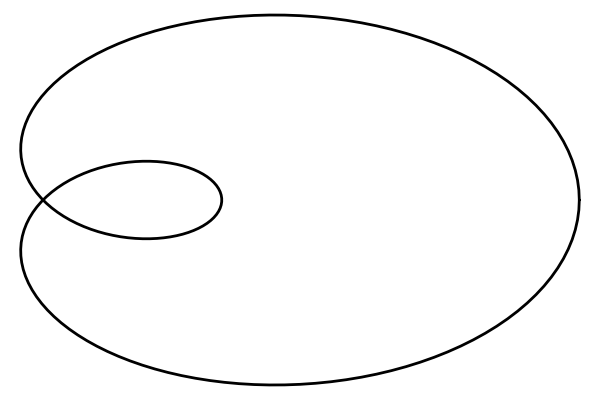
\includegraphics[width=\linewidth]{./assets/3-1-1/limacon-a-gt-1.png}
    \caption{$|a|>1$}
  \end{subfigure}
  \begin{subfigure}[b]{0.3\linewidth}
    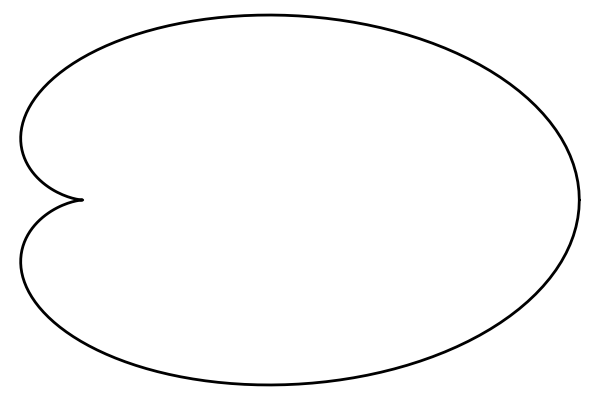
\includegraphics[width=\linewidth]{./assets/3-1-1/limacon-a-eq-1.png}
    \caption{$|a|=1$}
  \end{subfigure}  
  \begin{subfigure}[b]{0.3\linewidth}
    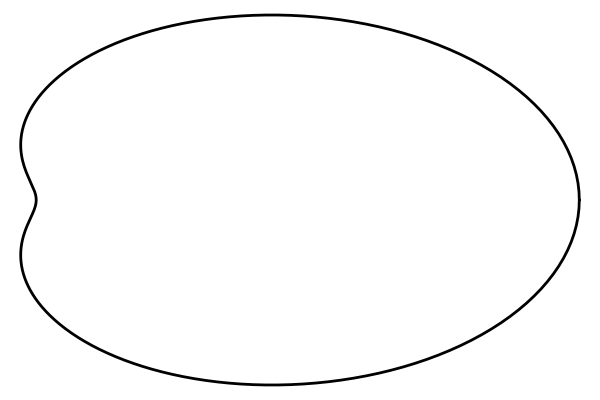
\includegraphics[width=\linewidth]{./assets/3-1-1/limacon-a-lt-1.png}
    \caption{$|a|<1$}
  \end{subfigure}
 
  \caption*{A limaçon (a) will degrade to a cardioid (b).}
\end{figure}

When $|a|>1$, $\gamma$ will have a self intersection. By definition, a simple closed curve is not to have any self-intersections.\\

Proof of self-intersection:\\
For some $t_0$ and $t_1$, $\gamma$ will have the same position if $\gamma$ has a self-intersection. Meaning,
$$
\gamma(t_0) \ = \ \gamma(t_1)
$$
but $t_0 \neq t_1$.

\end{document}
This is never printed